\documentclass[aspectratio=169, xcolor=table, 10pt]{beamer}

% -------------------------------------------------------------------
% Packages used in this document
% -------------------------------------------------------------------
\usepackage[no-math]{fontspec}
\usepackage[compatibility=false]{caption}
\usepackage{makecell}
\usepackage{ragged2e}
\usepackage{multicol}
\usepackage[utf8]{inputenc}
\usepackage{polyglossia}
\usepackage{amsmath}
\usepackage{hyperref}
\usepackage{amsfonts}
\usepackage{amssymb}
\usepackage{amsthm}
\usepackage{graphicx}
\usepackage{tikz}
\usepackage{hyperref}
\usepackage{qrcode}
\usetikzlibrary{calc}

% -------------------------------------------------------------------
% Font family, language settings
% -------------------------------------------------------------------
\setmainfont{MinionPro-Regular.otf}[
  Path = font/,
  BoldFont = MinionPro-Bold.otf,
  ItalicFont = MinionPro-It.otf,
  BoldItalicFont = MinionPro-BoldIt.otf
]
\setsansfont{MinionPro-Regular.otf}[
  Path = font/,
  BoldFont = MinionPro-Bold.otf,
  ItalicFont = MinionPro-It.otf,
  BoldItalicFont = MinionPro-BoldIt.otf
]
\newfontfamily\cyrillicfontsf{MinionPro-Regular.otf}[
  Path = font/,
  BoldFont = MinionPro-Bold.otf,
  ItalicFont = MinionPro-It.otf,
  BoldItalicFont = MinionPro-BoldIt.otf,
  Script = Cyrillic
]
\setmainlanguage{serbian}
\setotherlanguage{english}
% Increase default spacing between lines for 10%
\renewcommand{\baselinestretch}{1.1}
% Beamer template uses mono-font for URLs.
% Let's use the font that is already available
\renewcommand{\UrlFont}{\sffamily}

% -------------------------------------------------------------------
% Beamer settings: yellow theme
% -------------------------------------------------------------------
\usetheme{Madrid}
\usecolortheme{crane}

% This is that nice orange color used by Madrid/crane template
\definecolor{craneColor}{HTML}{FFBC00}

% Using plain text in bibliography, 'default' setting shows an ugly book icon
\setbeamertemplate{bibliography item}[text]

% Custom section page
\setbeamertemplate{section page}
{
  \setbeamertemplate{background}{\color{orange!20}\rule{\paperwidth}{\paperheight}}%
  \begin{frame}
    \begin{centering}
      \vfill

      % First line (above the rectangle)
      {\large\bfseries Део \thesection} \\[3ex]

      % Second line with background rectangle
      \begin{tikzpicture}
        \def\hmargin{0.25cm} % gap from left/right edges

        % Node with background rectangle and text
        \node[
          fill=craneColor,
          rounded corners=2mm,
          inner xsep=0.5cm,
          inner ysep=0.3cm,
          minimum width=\linewidth-2*\hmargin,
          align=center
        ] {\Large\insertsectionhead};
      \end{tikzpicture}

      \vfill
    \end{centering}
  \end{frame}
  \setbeamertemplate{background}{}%
}
% At the beginning of each section, show the section page
\AtBeginSection{\sectionpage}

% Custom table of contents template
% Just type \CustomTOC to generate TOC where appropriate
\newcommand{\CustomTOC}{
  \setbeamertemplate{background}{\color{orange!20}\rule{\paperwidth}{\paperheight}}%
  \begin{frame}[plain] % plain removes headers/footers for clean look
    \frametitle{Садржај}
    \vfill
    \setbeamertemplate{section in toc}[sections without number]
    \setbeamertemplate{section in toc}{
      \leavevmode\par
      \vspace{0.0em} % spacing between items
      \hspace{1em}
      {\color{red}\textbullet}~\inserttocsection
    }
    \setbeamerfont{section in toc}{size=\large, series=\bfseries}
    \setbeamercolor{section in toc}{fg=black}
    \tableofcontents[hideallsubsections]
    \vfill
  \end{frame}
  \setbeamertemplate{background}{}%
}

% -------------------------------------------------------------------
% Other settings
% -------------------------------------------------------------------
% URL that will be used for QR code generation
\newcommand{\MyQRurl}{https://github.com/saxon1964/hr-diag/tree/master/mathematica}

% Frame around images and charts
\setlength{\fboxrule}{0.5pt} % border thickness
\setlength{\fboxsep}{0.5pt}    % padding inside border


% -------------------------------------------------------------------
% General data about presentation
% -------------------------------------------------------------------
\title{Херцшпрунг-Раселов дијаграм}
\author{Лука Марковић}
\institute[МАТФ]{Математички факултет Универзитета у Београду}
\date{Септембар 2025.}

% -------------------------------------------------------------------
% Document begins here
% -------------------------------------------------------------------
\begin{document}

% Create title slide
\maketitle

% Create TOC using custom template
\CustomTOC

% ------------------------------------------------------------------
\section{Класификација звезда према површинској температури}
% ------------------------------------------------------------------

\begin{frame}{Какве све звезде постоје?}
  \begin{itemize}
    \item Не постоје две идентичне звезде.
    \item Звезде се разликују по маси, величини, површинској температури, боји, сјају и количини енергије коју емитују у јединици времена.
    \item Да ли је свака комбинација ових параметара могућа?
    \item Нека ограничења сигурно постоје: не постоје зелене или љубичасте звезде.
    \item Везе између наведених величина морају бити ”апсолутне”, независне од места посматрача.
    \item Нека својства звезда могуће је лако утврдити: типичан пример је боја звезде.
    \item Нека друга својства је много теже измерити.
    \item Тако, на пример, количина енергије коју звезда емитује зависи од њене величине и апсолутног сјаја.
    \item Са Земље, међутим, лако можемо да утврдимо само привидни сјај звезде.
    \item Привидни сјај звезде зависи од апсолутног сјаја али и од растојања на коме се звезда налази.
  \end{itemize}
\end{frame}

\begin{frame}{Класе звезда}
  \begin{itemize}
    \item Све звезде деле се на класе према тзв. Морган-Кинановом (MK) систему разрађеном на Харварду почетком XX века.\cite{britannica1}
    \item Класа звезде одређује се мерењем ширине карактеристичних Фраунхоферових линија водоника, хелијума, калцијума и титанијум-оксида у апсорпционом спектру звезде.
    \item Што је звезда топлија, ширина Фраунхоферових линија је већа.
    \item Прво су дефинисане класе \textbf{O}, \textbf{B}, \textbf{A}, \textbf{F}, \textbf{G}, \textbf{K} i \textbf{M}.
    \item Површинска температура звезде опада од класе \textbf{O} (најтоплије звезде) до \textbf{M} (најхладније).
    \item Свака класа има десет поткласа (0-9) у зависности од температуре. Сунце се налази у класи \textbf{G2}.
    \item Касније су додате класе \textbf{D} (бели патуљци), \textbf{L} i \textbf{T} (смеђи патуљци), \textbf{S} i \textbf{C} (угљеничне звезде).
    \item Овај систем користи се и даље али постоје и други, прецизнији, квантитативни системи.
  \end{itemize}
\end{frame}

\begin{frame}{Графички приказ звезданих класа}
  % In general, images can be displayed in a much simpler way.
  % The solution used here provides a caption that will not exceed the boundaries of the image
  \begin{figure}
    \centering
    % Frame image, then put it in the box
    \sbox0{\fbox{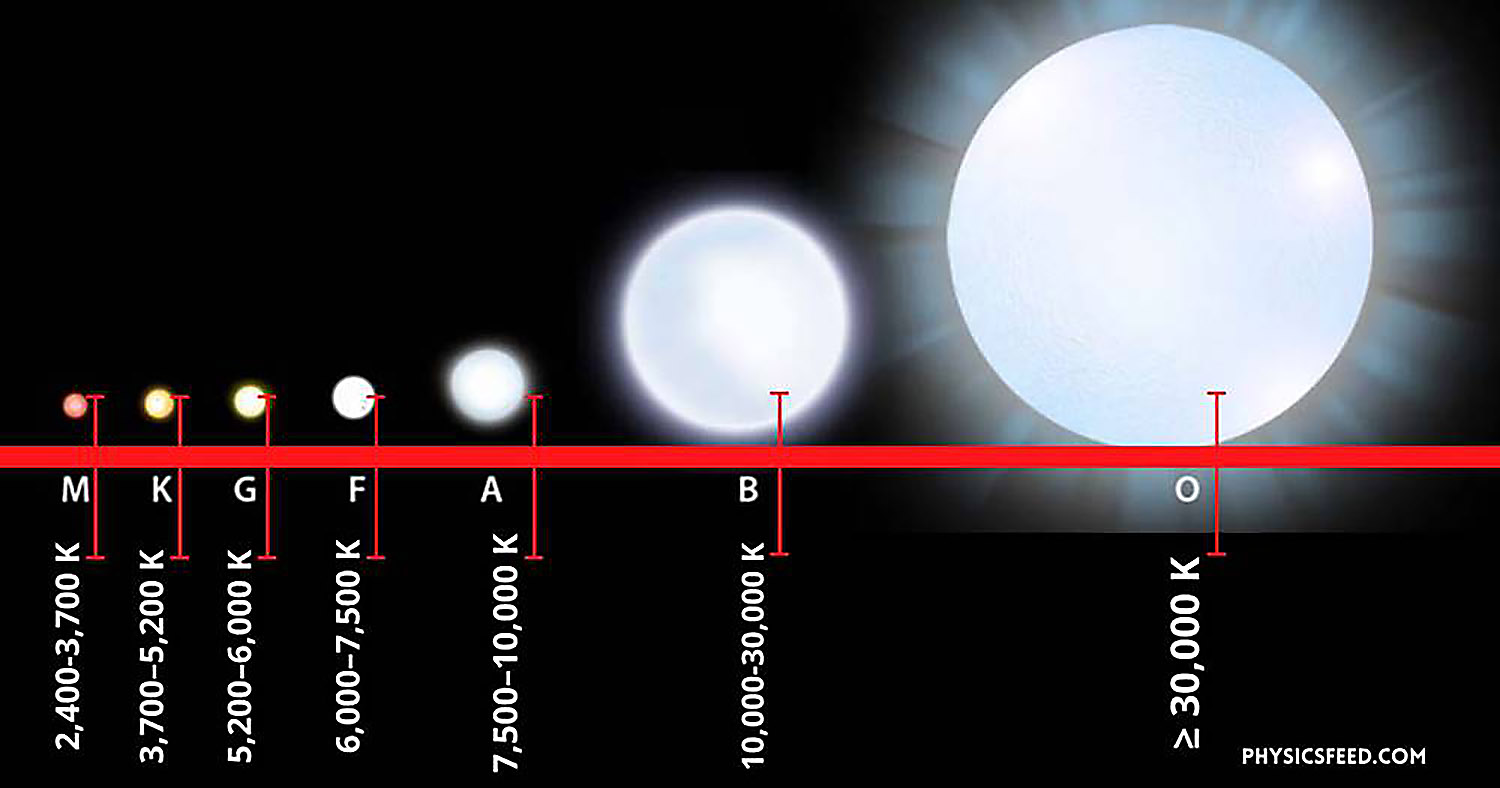
\includegraphics[height=0.65\textheight]{images/klase_zvezda.jpg}}}
    % Show the box!
    \usebox0
    % Set the caption width to the width of the box
    \captionsetup{width=\wd0}
    \caption{Главне спектралне класе са одговарајућим температурама, апроксимативним бојама и релативним величинама звезде}
  \end{figure}
\end{frame}

\begin{frame}{Индекс температуре звезде $B-V$}
  \begin{itemize}
    \item $B-V$ индекс одређује се посматрањем сјаја звезде кроз два филтера.
    \item $B$-индекс одређује се посматрањем сјаја звезде кроз $UB$-филтер осетљив на ултраљубичасту и плаву боју.
    \item $V$-индекс одређује се посматрањем сјаја звезде кроз $VB$-филтер осетљив на већи део видљивог спектра (плаву, жуту и зелену боју).
    \item $B-V$ индекс представља разлику ова два индекса. Систем је тако баждарен да звезда Вега има $B-V$ индекс једнак нули.
    \item Мање вредности индекса одговарају топлијим звездама, веће вредности хладнијим.
    \item $B-V$ индекс за Сунце износи 0,656, а за плавичасти Ригел -0,03.
    \item Из овог индекса може се директно израчунати температура површине звезде:
  \end{itemize}
  \begin{equation*}
    T=4600\text{K}\cdot\left[\frac{1}{0,92(B-V)+1,7}+\frac{1}{0,92(B-V)+0,62}\right]
  \end{equation*}
\end{frame}

\begin{frame}{Детаљи спектралне класификације}
  \begin{itemize}
    \item Класа звезде, њена температурa и индекс боје су три еквивалентне величине.
  \end{itemize}
  \begin{table}
    \vspace{-1em}
    \resizebox{\textwidth}{!}{
      \begin{tabular}{|c|c|c|c|c|>{\RaggedRight}p{4cm}|c|}
      \hline
      \rowcolor{craneColor}
        \textbf{\textcolor{black}{Класа}} &
        \textbf{\textcolor{black}{Температура (K)}} &
        \textbf{\textcolor{black}{Боја}} &
        \textbf{\textcolor{black}{Маса ($M_\odot)$}} &
        \textbf{\textcolor{black}{\makecell{Водоничне линије \\ спектра}}} &
        \textbf{\textcolor{black}{\makecell[l]{Друге линије \\ спектра}}} &
        \textbf{\textcolor{black}{\makecell{Проценат \\ звезда}}} \\
      \hline
      \hline
      \rowcolor{orange!15}\textbf{O} & > 33.000 & плава & > 16 & слабе & вишеструко јонизовани атоми & ~0,0003\% \\
      \hline
      \rowcolor{orange!25}\textbf{B} & 10.000 - 33.000 & плава/бела & 2,1 - 16 & средње & неутрални хелијум & ~0,1\% \\
      \hline
      \rowcolor{orange!15}\textbf{A} & 7.500 - 10.000 & бела/плава & 1,4 - 2,1 & јаке & јонизовани калцијум, неутрални хелијум & ~0,6\% \\
      \hline
      \rowcolor{orange!25}\textbf{F} & 6.000 - 7.500 & бела & 1,0 - 1,4 & средње & јонизовани калцијум, метали & ~3\% \\
      \hline
      \rowcolor{orange!15}\textbf{G} & 5.200 - 6.000 & жута & 0,8 - 1,0 & слабе & јаке линије метала & ~7,5\% \\
      \hline
      \rowcolor{orange!25}\textbf{К} & 3.700 - 5.200 & жута/оранж & 0,45 - 0,8 & врло слабе & неутрални калцијум, титан-оксид & ~12\% \\
      \hline
      \rowcolor{orange!15}\textbf{М} & < 3.700 & оранж/црвена & < 0,45 & врло слабе & јаке линије калцијума и титан-оксида, неутрални метали & ~76\% \\
      \hline
      \end{tabular}
    }
  \end{table}
\end{frame}

% ------------------------------------------------------------------
\section{Привидни сјај и магнитуда звезде }
% ------------------------------------------------------------------

\begin{frame}{Привидни сјај}
  \begin{columns}[T]
    \begin{column}{0.35\textwidth}
      \begin{figure}
        \centering
        \sbox0{\fbox{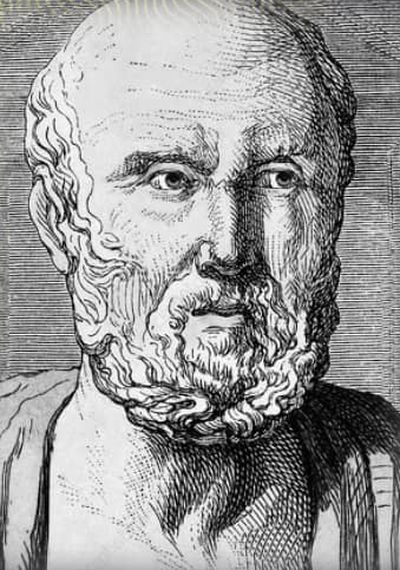
\includegraphics[height=0.60\textheight]{images/hiparh.jpg}}}
        \usebox0
        \captionsetup{width=\wd0}
        \caption{Хипарх, највећи антички астроном}
      \end{figure}
    \end{column}
    \begin{column}{0.65\textwidth}
      \begin{itemize}
        \item Довољан је један поглед на ноћно небо па да утврдимо да звезде сјаје различитим интензитетом.
        \item Хипарх је 135. године п.н.е направио каталог са 850 звезда у коме је свакој звезди доделио број од 1 до 6, у зависности од сјаја (магнитуде).
        \item Најсјајније звезде имале су ознаку 1 док су оне једва видљиве имале ознаку 6.
        \item Развој телескопа и фотометрије омогућио је да се сјај звезда објективно измери.
        \item У исто време утврђено је да људско око детектује промене у интензитету светлости по логартиамској скали.
        \item Такође је утврђено да звезде са ознаком 1 имају 100 пута већи сјај од звезде са ознаком 6.
      \end{itemize}
    \end{column}
  \end{columns}
\end{frame}

\begin{frame}{Савремена скала звезданих магнитуда}
  \begin{itemize}
    \item Хипархов систем, уз незнатне измене, користи се и данас!
    \item Суштински, користи се чињеница да, према Хипарховој логаритамској скали, разлика у магнитуди величине 5 одговара 100 пута јачем или слабијем интензитету светлости.
    \item То значи да је звезда која има магнитуду за један број мању од друге сјајнија од ње $\sqrt[5]{100}\approx2,5$ пута.
    \item Хипархов систем у међувремену je рекалибрисан:
    \begin{itemize}
      \item Звезда Вега има магнитуду 0.
      \item Задржано је старо емпиријско правило да 100 пута сјајнија (тамнија) звезда има магнитуду мању (већу) за 5.
    \end{itemize}
  \item С обзиром да на небу постоје објекти сјајнији од Веге (Сунце, Месец, Венера, Сиријус...), њихова магнитуда је негативна!
  \item Овако измерене магнитуде називају се \textbf{привидним} јер зависе од растојања посматраног објекта од нас.
  \end{itemize}
\end{frame}

\begin{frame}{Сјај неких небеских тела}
  \begin{multicols}{2}
    \begin{itemize}
      \item Сунце: -26,5
      \item Пун Месец: -12,5
      \item Венера: -4,3
      \item Марс и Јупитер: -3
      \item Меркур: -2
      \item Сиријус: -1,44
      \item Вега, Сатурн: 0
      \item Антарес: 1
      \item Северњача: 2
      \item Уран: 5
      \item Лимит голог ока: 6,5
      \item Церес: 7
      \item Нептун: 8
      \item Лимит двогледа: 10
      \item Проксима кентаури: 11,1
      \item Плутон: 14
      \item Лимит телескопа (8m): 28
      \item Лимит телескопа ”Хабл”: 32
    \end{itemize}
  \end{multicols}
\end{frame}

% ------------------------------------------------------------------
\section{Апсoлутна магнитуда и луминозност звезде}
% ------------------------------------------------------------------

\begin{frame}{Апсолутна магнитуда (сјај) звезде}
  \begin{itemize}
    \item Привидна магнитуда не говори много о количини енергије коју звезда емитује\cite{wiki1}. Неке звезде изгледају сјајније јер су нам ближе а не зато што емитују велику количину енергије.
    \item Зато је неопходно увести апсолутну магнитуду (сјај) која зависи само од снаге звезданог извора енергије.
    \item Апсолутна магнитуда дефинисана је као привидна магнитуда измерена са растојања од 10 парсека (1 парсек $\approx$ 3.26 светлосних година).
    \item Означимо апсолутну магнитуду са $M$, привидну магнитуду са $m$ а наше растојање до звезде мерено у парсецима са $d_{pc}$.
    \item Када се узме у обзир да енергетски флукс звезде опада са квадратом растојања и да 100 пута сјајнији светлосни извор има магнитуду мању за 5, добија се следећа једначина:
      \begin{equation*}
        M=m-5(\log_{10}d_{pc} - 1)
      \end{equation*}
    \item Одређивање апсолутне магнитуде своди се на мерење растојања до светлосног извора $d_{pc}$.
  \end{itemize}
\end{frame}

\begin{frame}{Луминозност}
  \begin{itemize}
    \item По дефиницији, луминозност звезде $L$ представља количину енергије коју звезда емитује у јединици времена.
    \item Уместо апсолутне вредности, луминозност се најчешће исказује релативно у односу на луминозност Сунца $L_\odot$.
    \item Ако апсолутну магнитуду звезде означимо са $M$ а апсолутну магнитуду Сунца са $M_\odot$, онда се релативна луминозност звезде може срачунати формулом:
      \begin{equation*}
        \frac{L}{L_\odot} = 100^\frac{M_\odot-M}{5}
      \end{equation*}
    \item Референтне вредности за Сунце су: $L_\odot=3,84\times 10^{26}\text{W}$, $M_\odot=4,75$. Нижим апсолутним магнитудама одговара већа луминозност (снага) звезде.
    \item Многе звезде имају много нижу апсолутну магнитуду од Сунца, самим тим и много већу луминозност: Бетелгез (-5,6), Наос (-6,0), Ригел (-7,0), Денеб (-7,2), Сиријус (1,4)...
  \end{itemize}
\end{frame}

\begin{frame}{Израчунавање радијуса звезде}
  \begin{itemize}
    \item Приметимо да се на основу познате површинске температуре звезде (њене класе) и луминозности (апсолутне магнитуде), лако може одредити и величина звезде.
    \item Према Штефан-Болцмановом закону, емисиона моћ апсолутно црног тела, дефинисана као количина енергије $j^*$ коју емитује јединица површине тела температуре $T$ у јединици времена дата је једначином:
      \begin{equation*}
        j^*=\sigma T^4
      \end{equation*}
    \item Симбол $\sigma$ означава Штефан-Болцманову константу која износи $5.6704\cdot 10^{-8}\textrm{W}\textrm{m}^{-2}\textrm{K}^{-4}$.
    \item Пошто луминозност $L$ представља укупну снагу звезде чија ја површина $A$ следи да је њен порлупречник $R$:
      \begin{equation*}
        L=j^*A=\sigma T^4 \cdot 4R^2\pi\implies R=\sqrt{\frac{L}{4\sigma T^4\pi}}=\frac{1}{2T^2}\sqrt{\frac{L}{\sigma\pi}}
      \end{equation*}
  \end{itemize}
\end{frame}

% ------------------------------------------------------------------
\section{Мерење звезданих растојања}
% ------------------------------------------------------------------

\begin{frame}{Зашто је мерење растојања битно}
  \begin{itemize}
    \item На претходним слајдовима показано је како се на основу привидне магнитуде звезде и растојања до ње може израчунати апсолутна магнитуда звезде.
    \item Такође је показано како се из апсолутне магнитуде може израчунати луминозност звезде.
    \item Сходно томе, за одређивање луминозности звезде потребна су само два улазна податка: привидна магнитуда звезде и растојање до ње.
    \item Привидна магнитуда звезде мери се врло лако.
    \item Међутим, мерење растојања до звезда и галаксија далеко je компликованије.
    \item Данас се користи више различитих метода за мерење растојања у косммичком простору.
    \item Не постоји универзална метода која би се могла употребити у свим случајевима.
  \end{itemize}
\end{frame}

\begin{frame}{Метода паралаксе, концепт}
  \begin{figure}
    \centering
    \sbox0{\fbox{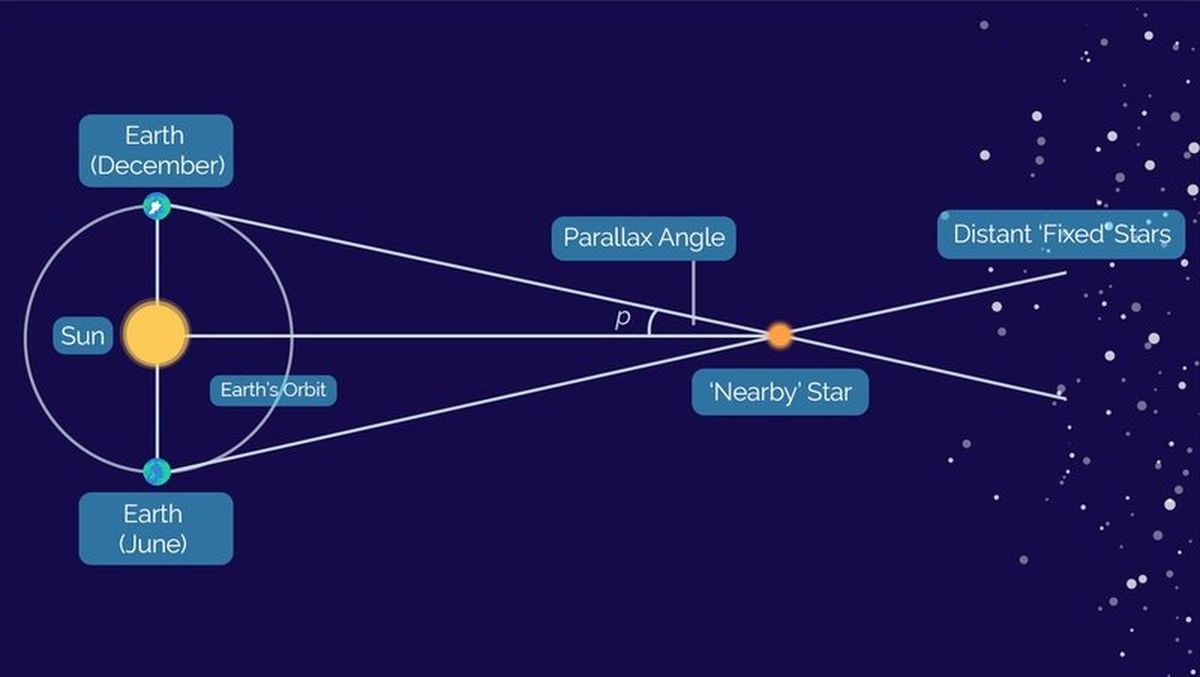
\includegraphics[height=0.70\textheight]{images/paralaksa.jpg}}}
    \usebox0
    \captionsetup{width=\wd0}
    \caption{Угао паралаксе приказан на слици у стварности је знатно мањи}
  \end{figure}
\end{frame}

\begin{frame}{Метода паралаксе, коришћење и примена}
  \begin{itemize}
    \item Звезде које се налазе врло далеко од нас изгледају потпуно непомично, без обзира на кретање Земље око Сунца.
    \item За релативно блиску звезду, промена тачке посматрања доводи до привидног померања звезде у односу на непомичну звездану позадину\cite{dina}.
    \item Осмотрено померање је највеће ако се посматрања врше у размаку од 6 месеци, са два супротна краја Земљине путање.
    \item Измерено померање представља двоструки угао паралаксе $p$ iz koga se moже израчунати растојање $d_{pc}$ до звезде:
      \begin{equation*}
        d_{pc}=\frac{1}{p}
      \end{equation*}
    \item Када је угао паралаксе у степенима, растојање до звезде изражено је у парсецима.
    \item Са Земље се може измерити паралакса не мања од 0.01 лучне секунде, помоћу телескопа ”Хабл” граница се спушта до 0.001. Зато се метода паралаксе користи само за блиске звезде на растојању 100-1000 парсека, што је свега неколико процената пречника Млечног пута.
  \end{itemize}
\end{frame}

\begin{frame}{Цефеиде, променљиве звезде}
  \begin{columns}[T]
    \begin{column}{0.5\textwidth}
      \begin{figure}
        \centering
        \sbox0{\fbox{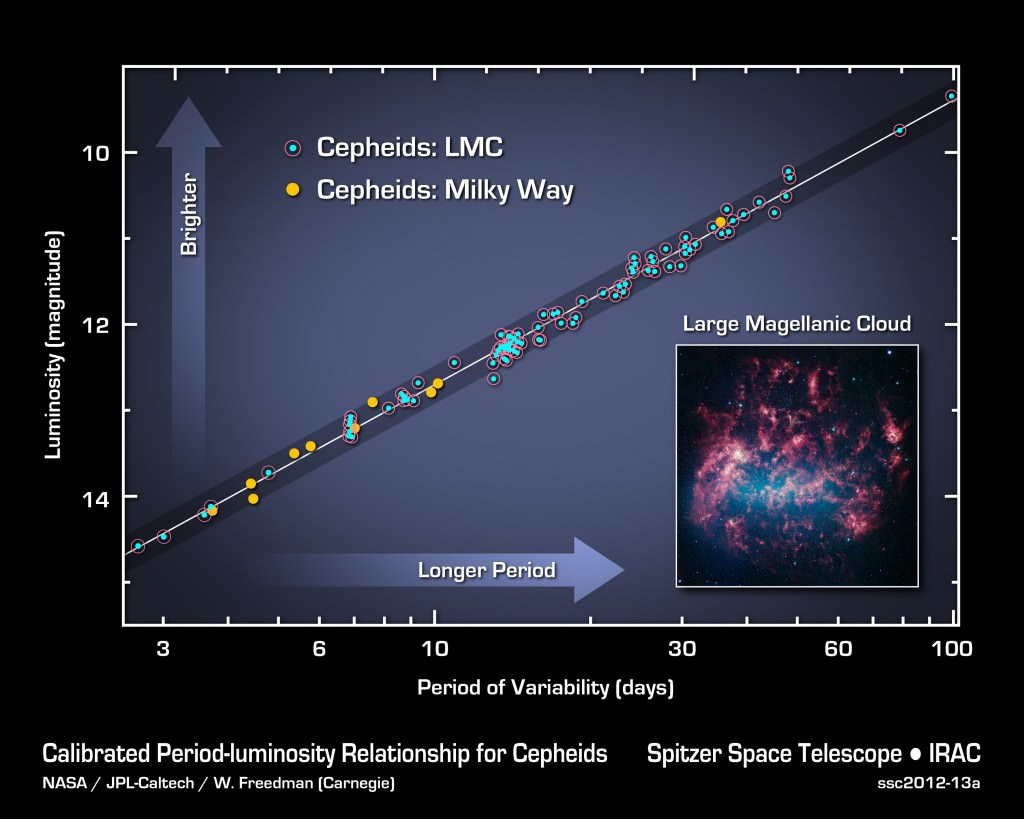
\includegraphics[height=0.55\textheight]{images/cefeide.jpg}}}
        \usebox0
        \captionsetup{width=\wd0}
        \caption{Линеарна веза између периода промене сјаја и луминозности за цефеиде унутар Млечног пута и Великог Магелановог облака}
      \end{figure}
    \end{column}
    \begin{column}{0.5\textwidth}
      \begin{itemize}
        \item Звезде које током времена мењају свој сјај називају се променљивим звездама.
        \item У ту групу спадају и цефеиде чији се сјај мења врло правилно, са периодом који износи од једног до 100 дана.
        \item Током једног циклуса цефеиде мењају луминозност (апсолутну магнитуду), полупречник и температуру.
        \item Оно што цефеиде чини тако специјалним је чињеница да постоји линеарна веза између њихове луминозности (којој одговара апсолутна магнитуда) и периода.
      \end{itemize}
    \end{column}
  \end{columns}
\end{frame}

\begin{frame}{Зашто су цефеиде важне?}
  \begin{itemize}
    \item Постоји линеарна веза између луминозности цефеида (којој одговара апсолутна магнитуда) и периода промене сјаја.
    \item Период и привидни сјај цефеиде су лако мерљиве величине. Из периода се може израчунати луминозност а на основу ње и апсолутна магнитуда.
    \item На основу релативне и апсолутне магнитуде лако се може израчунати растојање до звезде.
    \item Рачуницу компликује чињеница да постоје две фамилије цефида са различитим нагибима линије период-луминозност. Пажљивим посматрањем могуће је утврдити којој фамилији припада посматрана цефеида.
    \item Многе цефеиде су велике, веома светле звезде, могуће их је идентификовати не само у Млечном путу него и у суседним галаксијама.
    \item Земаљски телескопи могу да уоче цефеиде све до удаљености од 13 милиона светлосних година. Космички телескоп ”Хабл” успешно је идентификовао цефеиде на растојању од 56 милиона светлосних година.
  \end{itemize}
\end{frame}

\begin{frame}{Бели патуљци и супернове типа Ia}
  \begin{columns}[T]
    \begin{column}{0.7\textwidth}
      \begin{figure}
        \centering
        \sbox0{\fbox{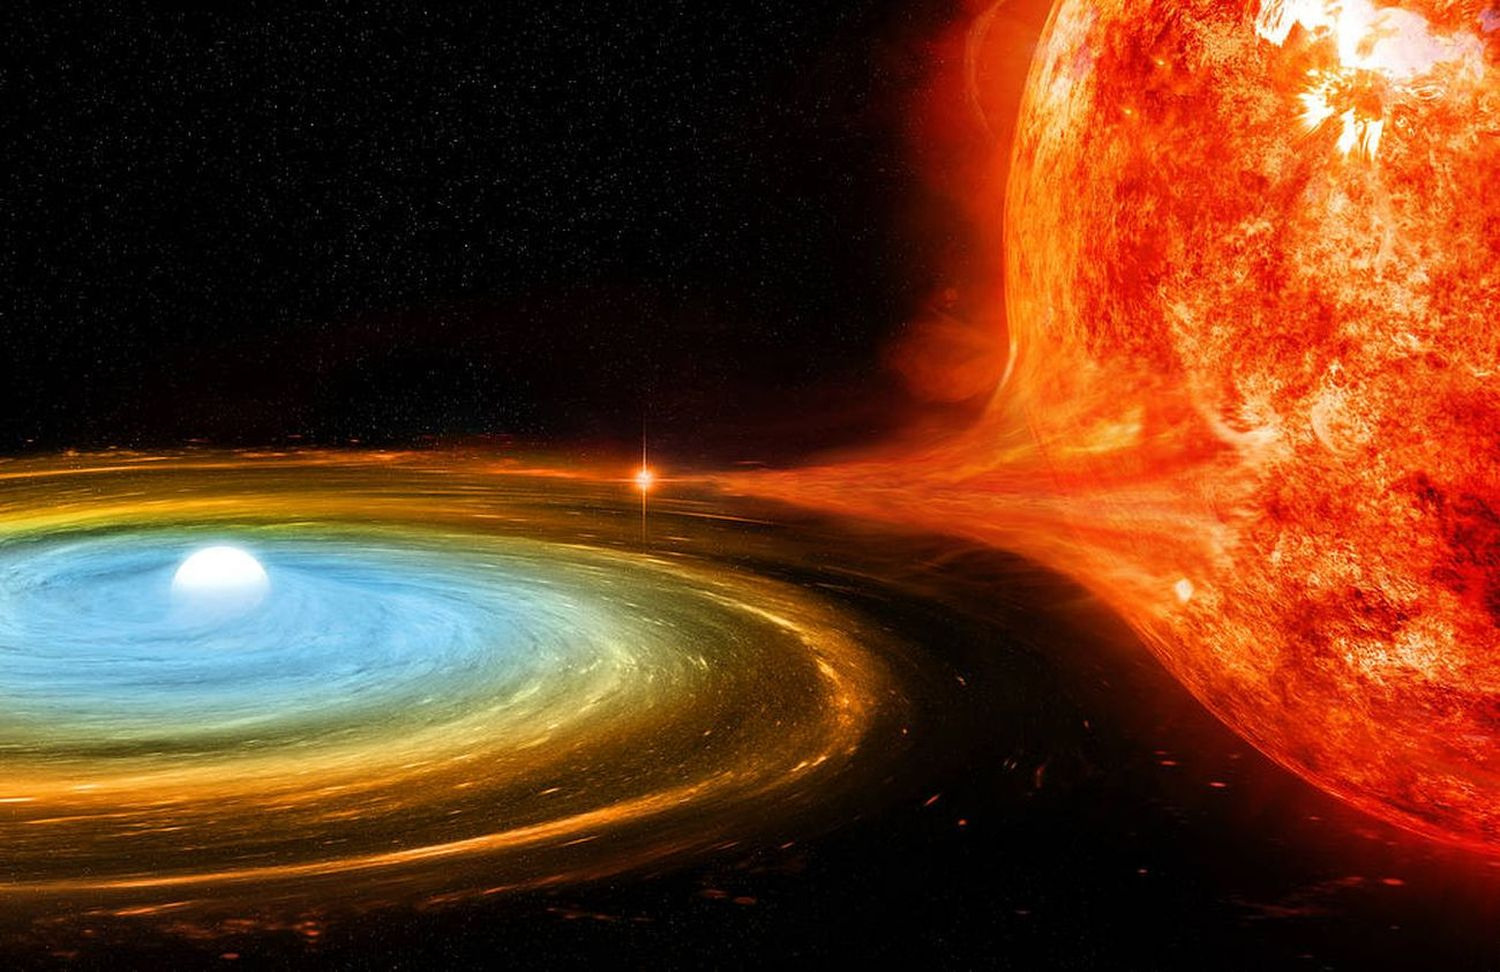
\includegraphics[width=0.95\textwidth]{images/beli_patuljak.jpg}}}
        \vspace{-1em}
        \usebox0
      \end{figure}
    \end{column}
    \begin{column}{0.3\textwidth}
      Бинарни систем у коме бели патуљак преузима материју од суседне звезде. Када маса белог патуљка пређе границу од $1.44 M_{\odot}$, могућа је експлозија супернове типа Ia.
    \end{column}
  \end{columns}
\end{frame}

\begin{frame}{Специфичности супернове типа Ia}
  \begin{itemize}
    \item Мале и средње звезде завршавају свој живот као бели патуљци.
    \item Реч је о топлом језгру звезде која је потрошила нуклеарно гориво и одбацила спољне слојеве.
    \item Бели патуљак има екстремну густину. Претежно је сачињен од угљеника и кисеоника.
    \item Иако су бели патуљци релативно мали, гравитационо поље у њиховој близини екстремно je јако.
    \item Ако је бели патуљак део двојног звезданог система, бели патуљак мoже да почне да ”краде” материју од суседне звезде. Када маса белог патуљка пређе границу од $1.44 M_{\odot}$, притисак у средишту постаје толико велики да отпочиње нуклеарна реакција.
    \item У свега пар секунди бели патуљак ће фузионисати скоро сав угљеник и кисеоник у теже елементе. Притом се генерише енергија упоредива са енергијом читаве галаксије.
    \item Настаје супернова типа Iа чија ће експлозија потпуно уништити бинарни систем.
    \item Све супернове типа Iа имају исту апсолутну магнитуду: \textbf{-19.3}. На основу привидног сјаја и апсолутне магнитуде може се израчунати даљина белог патуљка.
    \item Овом методом могу се мерити растојања од више милијарди светлосних година.
  \end{itemize}
\end{frame}

% ------------------------------------------------------------------
\section{Херцшпрунг-Раселов дијаграм}
% ------------------------------------------------------------------

\begin{frame}{Најважнији дијаграм савремене астрономије}
  \begin{columns}[T]
    \begin{column}{0.45\textwidth}
      \begin{figure}
        \centering
        \sbox0{\fbox{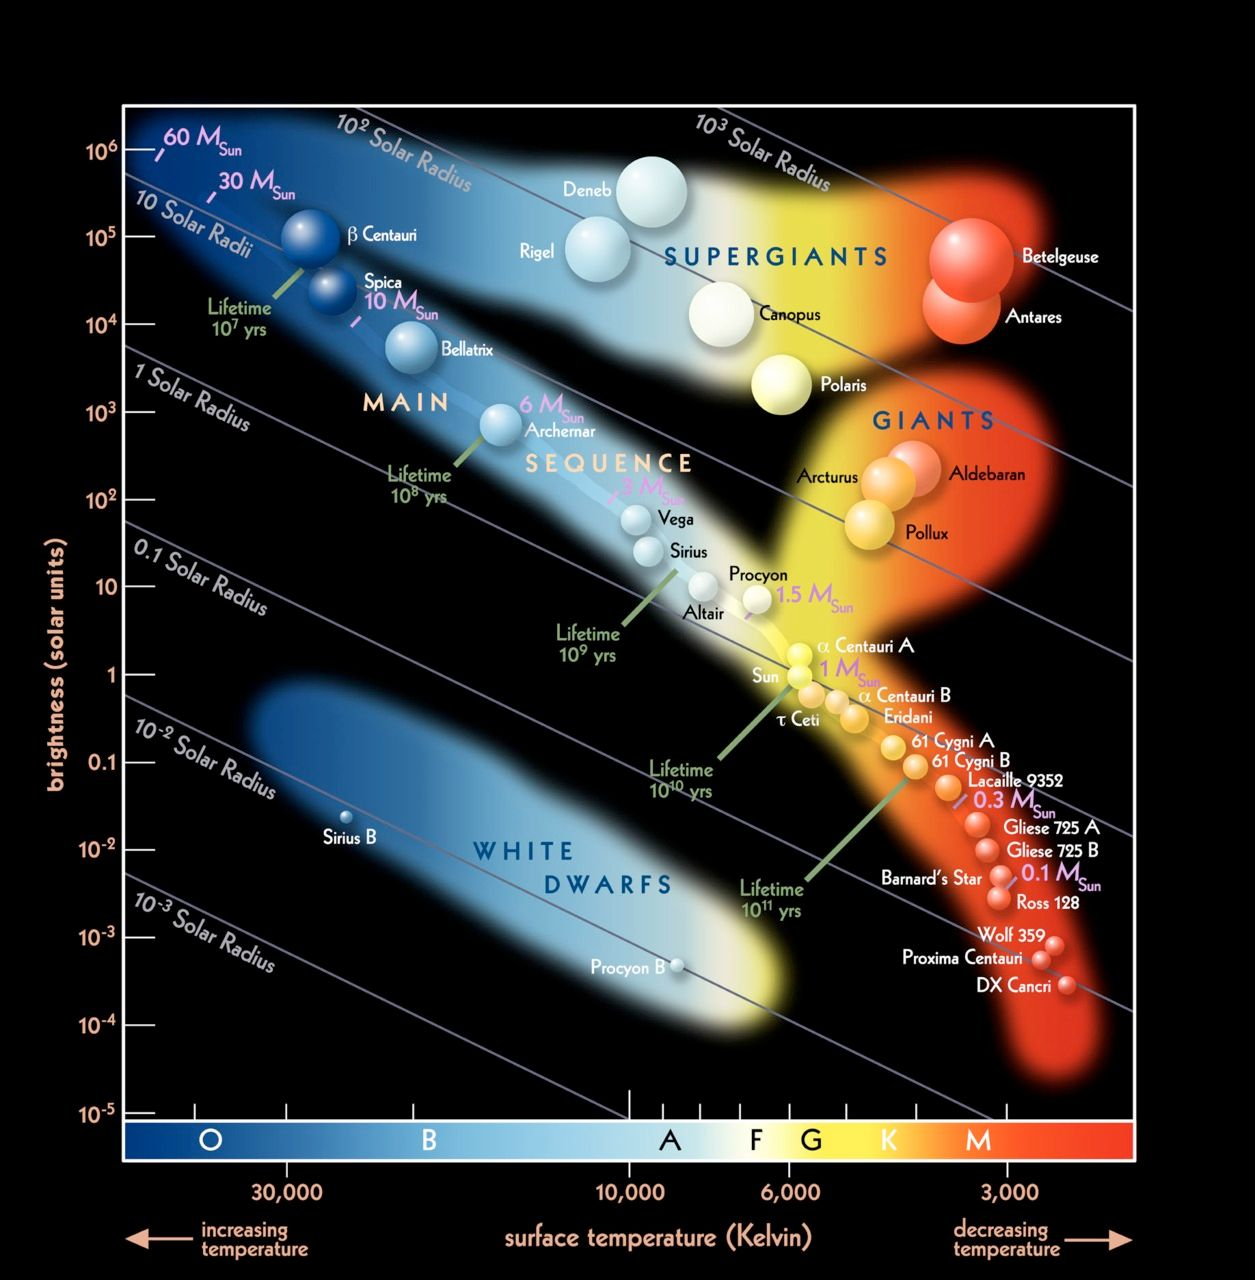
\includegraphics[height=0.8\textheight]{images/hr.jpg}}}
        \vspace{-1em}
        \usebox0
      \end{figure}
    \end{column}
    \begin{column}{0.55\textwidth}
      \begin{itemize}
        \item Херцшпрунг-Раселов (H-R) дијаграм представља, по много чему, најважнији дијаграм у астрономији због улоге коју има у проучавању еволуције звезда.
        \item Дијаграм су, независно један од другог, креирали Ејнар Херцшпрунг и Хенри Норис Расел почетком XX века\cite{mathias}.
        \item Постоји неколико форми овог дијаграма али су у суштини све оне међусобно еквивалентне.
        \item У својој изворној верзији, H-R дијаграм представља зависност луминозности звезде од њене површинске температуре.
        \item Дијаграм лево илуструје положај различитих типова звезда на H-R дијаграму.
      \end{itemize}
    \end{column}
  \end{columns}
\end{frame}

\begin{frame}{Еквивалентни облици H-R дијаграма}
  \begin{itemize}
    \item На претходним слајдовима утврдили смо да постоји корелација између класе звезде, индекса B-V и површинске температуре звезде.
    \item Свака од ове три величине може да представља апсцису H-R дијаграма.
    \item Takoђе смо утврдили да постоји директна веза између луминозности и апсолутне магнитуде звезде.
    \item Било која од ове две величине може да предствља ординату H-R дијаграма.
    \item Површинске температуре крећу се између 3.000 и 50.000 келвина. Иако распон температура обухвата само два реда величине, за апсцису се најчешће се користи логаритамска скала.
    \item Разлика у луминозности звезда много је већа (најмање десет редова величине) тако да је ордината увек логаритамска.
    \item Из чисто историјских разлога, апсциса је ”обрунта”: пoвршинска температура звезде опада са десна у лево.
  \end{itemize}
\end{frame}

\begin{frame}{Како је настао H-R дијаграм?}
  \begin{columns}[T]
    \begin{column}{0.4\textwidth}
      \begin{figure}
        \centering
        \sbox0{\fbox{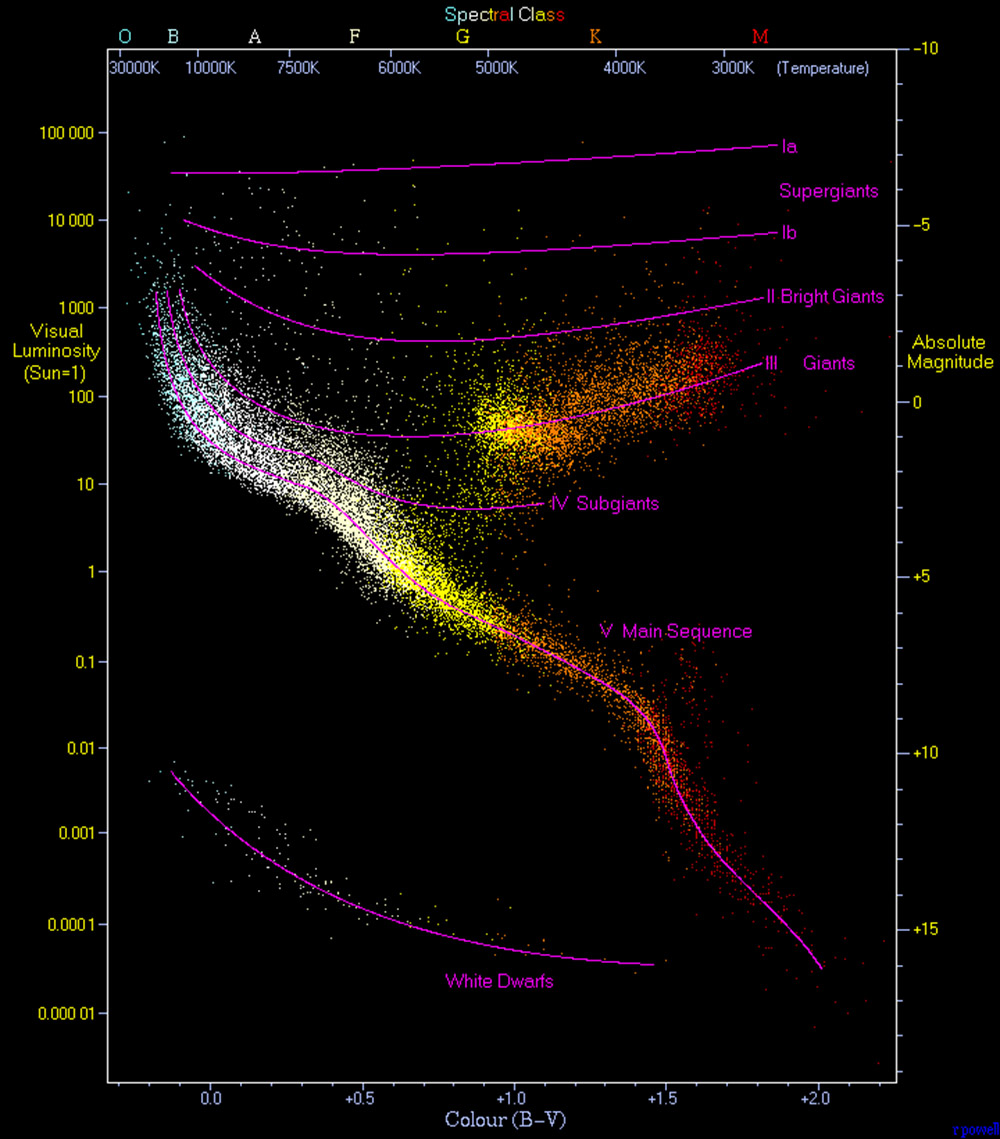
\includegraphics[height=0.8\textheight]{images/hr-2.jpg}}}
        \vspace{-1em}
        \usebox0
      \end{figure}
    \end{column}
    \begin{column}{0.6\textwidth}
      \begin{itemize}
        \item Звезде током времена мењају своју температуру и луминозност, самим тим и положај на H-R дијаграму.
        \item Због спорости промена, дијаграм није настао праћењем појединачних звезда током времена већ уцртавањем звезда мерењем њиховог тренутног стања.
        \item Дијаграм је касније допуњен подацима из два велика звездана каталога: ”Hiparcos” и ”Gliese”.
        \item Тако је настао дијаграм на левој страни који садржи податке за око 20.000 звезда.
        \item Дијаграм приказује звезде у разним фазама њихове еволуције.
      \end{itemize}
    \end{column}
  \end{columns}
\end{frame}

\begin{frame}{Елементи H-R дијаграма}
  \begin{itemize}
    \item Најуочљивији део дијаграма, тзв. ”Главни низ” простире се дијагонално, од горњег левог до доњег десног угла.
    \item Бројност звезда драстично расте како се спуштамо низ главни низ, од плавих, екстремно топлих и великих звезда до релативно хладних и тамних.
    \item Када млада звезда започне да фузионише водоник у хелијум, она заузме почетно место негде у главном низу. У том низу, звезда проведе око 90\% свог живота.
    \item Када звезда потроши своје водонично гориво, површинска температура опада али запремина драстично расте: звезда прелази у горњи део дијаграма у коме се налазе плави и црвени џинови и супер-џинови, звезде у задњим стадијумима еволуције.
    \item Звезде мале величине завршавају свој живот као бели патуљци (на дијаграму се налазе испод главног низа), оне веће као супернове иза којих остају неутронске звезде или црне рупе.
  \end{itemize}
\end{frame}

\begin{frame}{Неке особине H-R дијаграма}
  \begin{itemize}
    \item Дијаграм показује да природа не уме да створи звезде произвољне температуре и луминозности. Највећи део дијаграма је празан.
    \item Утврђено је да за звезде у главном низу постоји директна веза између луминозности $L$ и масе звезде $M$:
      \begin{equation*}
        \frac{L}{L_\odot}=\left(\frac{M}{M_\odot}\right)^\alpha,\quad \alpha\approx 3,5
      \end{equation*}
    \item Из положаја звезде на дијаграму може се закључити у којој фази свог животног циклуса се звезда налази.
    \item H-R дијаграм се користи и као универзални ”даљинар”: анализом спектра можемо да утврдимо да се звезда налази у главном низу и да има одређену класу. Из класе се може одредити температура а на основу ње се са H-R дијаграма очита њена луминозност, тј. апсолутна магнитуда. Из привидне и апсолутне магнитуде лако се срачуна растојање до звезде.
    \item Сличан поступак може се спровести и за звезде изван главног низа али је рачуница компликованија.
  \end{itemize}
\end{frame}

\begin{frame}{Конструкција H-R дијаграма коришћењем програма "Mathematica"}
  \begin{itemize}
    \item ”Mathematica" од верзије 10 има могућност да са ”Mathematica” сервера преузме податке за преко 400.000 звезда. То омогућава функција \textbf{StarData[]}.
    \item Количина расположивих података варира од звезде до звезде.
    \item Пажљивим филтрирањем података могуће је пронаћи око 75.000 звезда за које је дефинисана и површинска температура и луминозност.
    \item На основу ових података могуће је нацртати H-R дијаграм чији се финални облик у потпуности слаже са дијаграмима који су начињени коришћењем неупоредиво већег узорка.
    \item Дијаграм не изгледа као да садржи 75.000 тачака али то је последица чињенице да су подаци о звездама врло грубо заокружени тако да се вредности врло често поклапају.
    \item Дијаграм се може учинити ”интересантнијим” тако што се температура и луминозност звезде пре цртања помноже неким бројем из сегмента $[1-x,1+x]$, где је $x$ нека мала вредност.
    \item Оригинални ”Mathematica Notebook” фајл са изворним кодом може се преузети са линка који је уцртан на сам дијаграм на следећем слајду.
  \end{itemize}
\end{frame}

\begin{frame}{H-R дијаграм нацртан коришћењем програма ”Mathematica”}
  \centering
  \vspace{0.5em}
  \fbox{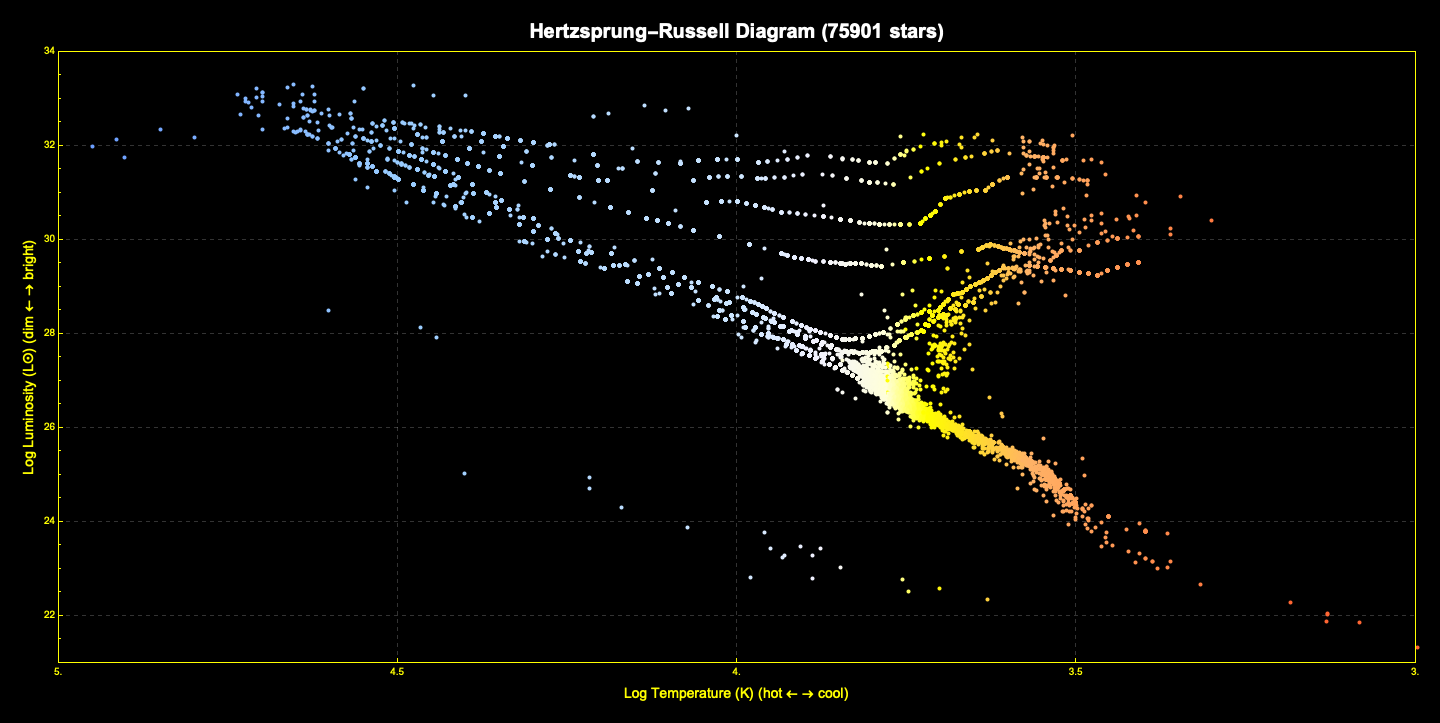
\includegraphics[width=0.9\textwidth,height=0.80\textheight]{images/hr.png}}
  % show QR code from slide 2 onward, bottom-left corner
  \uncover<2->{%
    \begin{tikzpicture}[remember picture,overlay]
      \node[anchor=south west, xshift=1.9cm, yshift=1.5cm,
        inner sep=3pt, fill=white, rounded corners=2pt]
        at (current page.south west)
        {\qrcode[height=2cm]{\MyQRurl}};
    \end{tikzpicture}
  }
\end{frame}

% ------------------------------------------------------------------
\section{Закључак}
% ------------------------------------------------------------------

\begin{frame}{Значај Херцшпрунг–Раселовог дијаграма}
  \begin{itemize}
    \item Приказује однос између луминозности (апсолутне магнитуде) и температуре (спектралне класе звезда).
    \item Доказује да главна својства звезда нису потпуно произвољна, напротив: постоји јака корелација између њих.
    \item Омогућава класификацију звезда у неколико главних група: главни низ, џинови, суперџинови и бели патуљци.
    \item Служи као алат за разумевање еволуције звезда – положај звезде на дијаграму одређује у којој фази живота се звезда налази.
    \item Омогућава процену старости и начин развоја звезданих јата и галаксија.
    \item Представља један од најважнијих инструмената у астрофизици јер повезује спољашња опажања са теоријом унутрашње грађе звезда.
    \item Омогућава мерење растојања до звезда где други методи нису на располагању.
  \end{itemize}
\end{frame}

% ------------------------------------------------------------------
% Bibliography
% ------------------------------------------------------------------
\begin{frame}{Референце}
    \begin{thebibliography}{9}

      \bibitem{britannica1}
      Britannica,
      \textit{Stellar Classification},
      \url{https://www.britannica.com/science/stellar-classification}

      \bibitem{wiki1}
      Wikipedia,
      \textit{Magnitude (astronomy)},
      \url{https://en.wikipedia.org/wiki/Magnitude_(astronomy)}

      \bibitem{dina}
      Dina Prialink,
      \textit{An Introduction to the Theory of Stellar Structure and Evolution},
      Cambridge University Press, 2009, p. 3

      \bibitem{mathias}
      Mathias Scholz,
      \textit{The Physics of Stars: Structure, Evolution and Properties},
      Springer, 2025, pp. 28-29

    \end{thebibliography}
\end{frame}

\end{document}

